%----------------------------------------------------------------------------------------
%	PACKAGES AND OTHER DOCUMENT CONFIGURATIONS
%----------------------------------------------------------------------------------------

\documentclass[twoside,twocolumn]{article}

\usepackage{blindtext} % Package to generate dummy text throughout this template 

\usepackage[T1]{fontenc} % Use 8-bit encoding that has 256 glyphs
\usepackage{microtype} % Slightly tweak font spacing for aesthetics
\usepackage[utf8]{inputenc}
\usepackage{indentfirst}

\usepackage[english]{babel} % Language hyphenation and typographical rules

\usepackage[hang, small,labelfont=bf,up,textfont=it,up]{caption} % Custom captions under/above floats in tables or figures
\usepackage{booktabs} % Horizontal rules in tables
\usepackage{multirow}
\usepackage{float} % For using H in positioning


\usepackage{enumitem} % Customised lists

\usepackage{abstract} % Allows abstract customisation
\renewcommand{\abstractnamefont}{\normalfont\bfseries} % Set the "Abstract" text to bold

\usepackage{titlesec} % Allows customisation of titles
\renewcommand\thesection{\Roman{section}} % Roman numerals for the sections
\renewcommand\thesubsection{\roman{subsection}} % roman numerals for subsections
\titleformat{\section}[block]{\large\scshape\centering}{\thesection.}{1em}{} % Change the look of the section titles
\titleformat{\subsection}[block]{\large}{\thesubsection.}{1em}{} % Change the look of the section titles

\usepackage{titling} % Customising the title section

\usepackage{amsmath} % For equation alignment
\usepackage{amssymb} % For symbols in the equations

\usepackage{biblatex} %Imports biblatex package
\usepackage{csquotes}
\addbibresource{bibliography.bib} %Import the bibliography file

\usepackage{graphicx} % For images
\graphicspath{ {images/} }

\usepackage{appendix} % For appendices

%----------------------------------------------------------------------------------------
%	TITLE SECTION
%----------------------------------------------------------------------------------------

\setlength{\droptitle}{-4\baselineskip} % Move the title up

\title{Matrix-matrix Multiplication \\
    \large Characterisation and Analysis of the Performance On a Computing Platform} % Article title

\author{
João Alves\\[1ex] % Your name
\normalsize University of Minho \\ % Your institution
\normalsize a77070@alunos.uminho.pt % Your email address
\and % Uncomment if 2 authors are required, duplicate these 4 lines if more
Filipe Silva\\[1ex] % Second author's name
\normalsize University of Minho \\ % Second author's institution
\normalsize a77284@alunos.uminho.pt % Second author's email address
}
\date{} % Leave empty to omit a date
\renewcommand{\maketitlehookd}{%
\begin{abstract}

\textbf{
The goal of this project is to study the Roofline Model methodology, on the characterization of the performance bottlenecks, code profiling and its performance analysis, applying it to the matrix multiplication algorithm. The computing platform we worked with was a multicore processor, of the Universidade do Minho cluster SeARCH, more precisely the SeARCH 662 nodes.
}

\end{abstract}
}

%----------------------------------------------------------------------------------------

\begin{document}

% Print the title
\maketitle

%----------------------------------------------------------------------------------------
%	ARTICLE CONTENTS
%----------------------------------------------------------------------------------------

\section{Introduction}

Nowadays, nearly almost desktop and server computers follow the same design. That is, besides the variations on the instruction sets, all of them use caches, pipelining, superscalar instruction issue, and out-of-order execution \cite{roofline}.

However, switching to multicore means that processors are a lot more diverse in terms of architecture and implementations, depending on the manufacturers which often ofter multiple products differing mainly on the number of cores.

So, it becomes the job of the programmer to better understand the different aspects of the platform's architecture. Therefore, models are designed to provide insights into the performance of the applications developed.

In this paper, we will focus on the performance of the matrix multiplication algorithm on a computing platform. Starting by developing a model to characterise the hardware environment, analyse bottlenecks and further study on the optimisations of the algorithm.

\section{Hardware Platform Characterisation}

In order to completely understand the performance of an algorithm, we first need to be fully aware of the resources offered by the hardware, so that it becomes possible to develop an analysis of the bottlenecks, limiting the performance of a certain kernel.

Since we used both our team's main laptop and a SeARCH cluster 662 node, we will perform an analysis into the hardware provided by both platforms, plotting the values into a Roofline Model.


\subsection{Team's Laptop Hardware Analysis}

The team's main laptop is a Dell XPS 15 9560 released in February 2017 (release tag 29Y07H2). It packs an Intel Core i7 7700HQ Kaby Lake processor and 8GB (2 slotsx4GB) of DDR4-2400MHz RAM. A more detailed view of the specifications and features implemented in the chip can be found in table \ref{tab:laptopspecs}.

\begin{table}[ht]
\resizebox{\columnwidth}{!}{%
\begin{tabular}{|l|r|}
\hline
\multicolumn{2}{|c|}{\textbf{Intel® Core™ i7-7700HQ Processor}}                          \\ \hline
Code Name                           & Kaby Lake                                          \\ \hline
\multicolumn{2}{|c|}{\textbf{Essentials}}                                                \\ \hline
Vertical Segment                    & Mobile                                             \\ \hline
Processor Number                    & i7-7700HQ                                          \\ \hline
\multicolumn{2}{|c|}{\textbf{Performance}}                                               \\ \hline
\# of Cores                         & 4                                                  \\ \hline
\# of Threads                       & 8                                                  \\ \hline
Processor Base Frequency            & 2.80 GHz                                           \\ \hline
Max Turbo Frequency                 & 3.80 GHz                                           \\ \hline
Bus Speed                           & 8 GT/s DMI                                         \\ \hline
\multicolumn{2}{|c|}{\textbf{Memory Specifications}}                                     \\ \hline
\multirow{2}{*}{Level 1 cache size} & 4 x 32 KB 8-way set associative instruction caches \\ \cline{2-2} 
                                    & 4 x 32 KB 8-way set associative data caches        \\ \hline
Level 2 cache size                  & 4 x 256 KB 4-way set associative caches            \\ \hline
Level 3 cache size                  & 6 MB 12-way set associative shared cache           \\ \hline
Max Memory Size                     & 64 GB                                              \\ \hline
Memory Types                        & DDR4-2400, LPDDR3-2133, DDR3L-1600                 \\ \hline
Max \# of Memory Channels           & 2                                                  \\ \hline
Max Memory Bandwidth                & 37.5 GB/s                                          \\ \hline
\multicolumn{2}{|c|}{\textbf{Advanced Technologies}}                                     \\ \hline
Intel® 64 ‡                         & Yes                                                \\ \hline
Instruction Set                     & 64-bit                                             \\ \hline
Instruction Set Extensions          & Intel® SSE4.1, Intel® SSE4.2, Intel® AVX2          \\ \hline
\end{tabular}
}
\caption{Team's laptop specifications \cite{cpuworld_laptopspecs} \cite{intel_laptopspecs}.}
\label{tab:laptopspecs}
\end{table}

In order to estimate the peak floating point performance (\textbf{PFP}) for single precision using the hardware specifications, it was considered that the width of the SIMD registers is 256 bits, hence 8 floats, and the throughput is one instruction per clock cycle. Also, because it is an architecture with FMA, we are able to perform fused multiply-adds. Multiplying that by the number of cores and the clock rate we came up with the following:

\begin{equation} \label{eq:pfplaptop}
\resizebox{\columnwidth}{!}{%
$\begin{aligned}
PFP & = \#cores \times frequency \times \frac{SIMD \thinspace width}{SIMD \thinspace throughput} \times FMA \\
    & = 4 \times 2.8 \times \frac{8}{1} \times 2 \\
    & = 179.2 \thinspace GFlops
\end{aligned}$
}
\end{equation}

Since this is an hardware limit, we can plot an horizontal line illustrating that the actual floating point performance can be no higher than the horizontal line.

Next, to measure the maximum streaming bandwidth, we used the STREAM benchmark obtaining a value of 36 GB/s for the peak memory bandwidth (\textbf{PMB}).

Finally, we are able to calculate the performance of the kernel as seen in equation \ref{eq:perf}. 

\begin{equation}
\label{eq:perf}
performance = min(PFP, \thinspace OP \times PMB)
\end{equation}

Figure \ref{fig:roofline} shows the plotted lines. These lines set an upper bound on performance of a kernel depending on it's operational intensity \cite{roofline}.

\begin{figure}[H]
    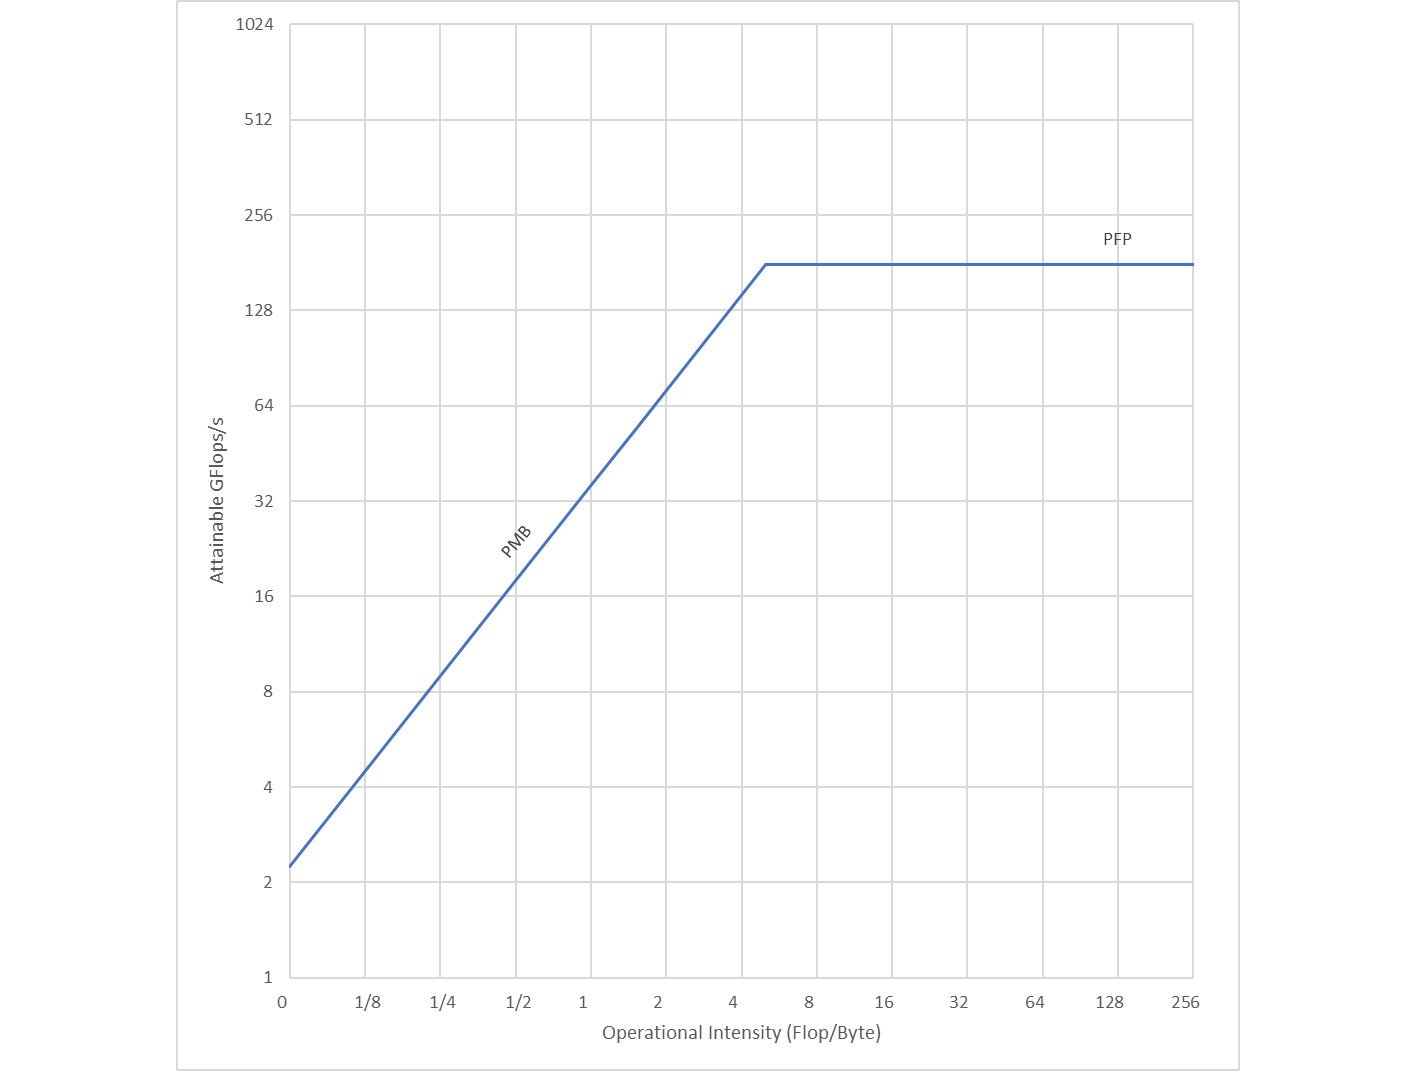
\includegraphics[width=\columnwidth]{laptop_roofline.png}
    \centering
    \caption{Roofline Model for our team's laptop.}
    \label{fig:roofline}
\end{figure}

\subsubsection{Addition of Ceilings}

Although the above values provide us with an upper bound to performance, this was obtained considering some optimisations are performed. In order to better understand which of them should be implemented first, we added the following ceilings ranking them from bottom to top, regarding the matrix multiplication kernel:

\begin{itemize}
    \item The lowest ceiling comes from using only one of the cores provided by the machine. There so, depending only on the clock rate being the single parameter in the equation. Thus, the first optimisation that could be applied is thread-level-parallelism (\textbf{TLP}), taking full advantage of the cores presented by the hardware.
    \item Second comes from exploiting vectorial instructions, that decrease the CPE of the kernel, given that we are able to perform the same operation over multiple data simultaneously. 
    \item The third appears from using FMA, to double the number of multiply-addition operations per cycle, because we are able to perform fused multiply-add operations.
    \item When it comes to memory ceilings, we were able to obtain a value of  16 GB/s for the peak memory bandwidth, using the STREAM benchmark compiled without any software optimisations.
\end{itemize}

At last, we ended up with the following Roofline Model, for our team's laptop.

\begin{figure}[H]
    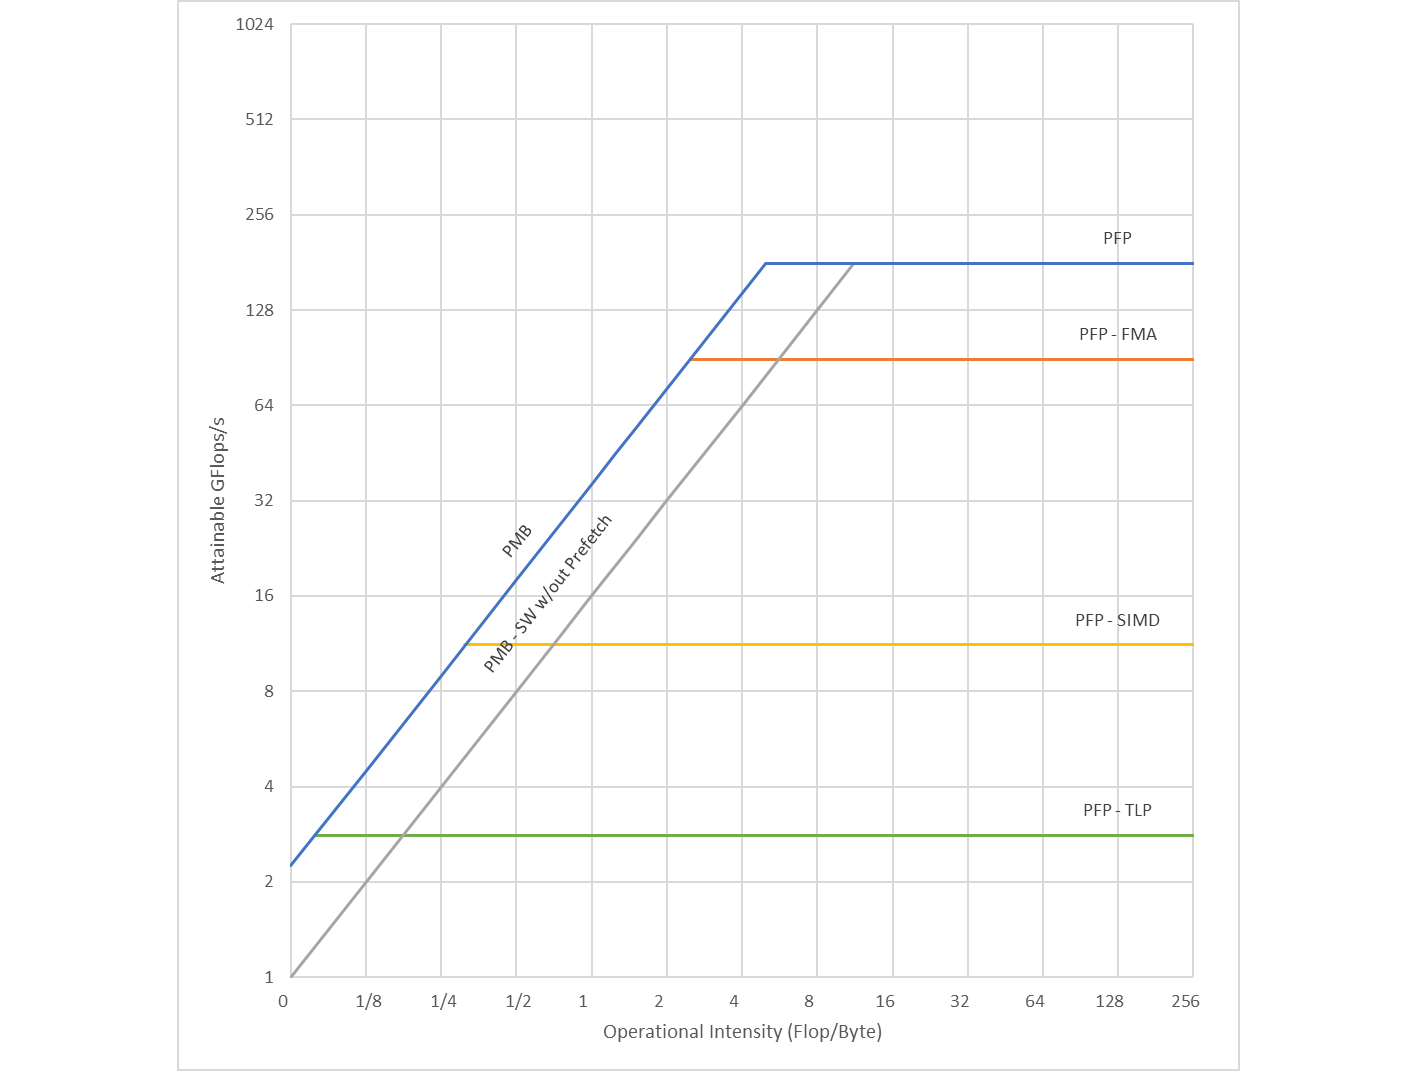
\includegraphics[width=\linewidth]{laptop_roofline_ceilings.png}
    \centering
    \caption{Roofline Model with ceilings for our team's laptop.}
    \label{fig:roofline_ceil}
\end{figure}

\subsection{SeARCH's Node Hardware Analysis}

The SeARCH's 662 nodes are dual processor machines, each an Intel Xeon Processor E5-2695 v2 Ivy Bridge \cite{search_nodes}. The more specific hardware features regarding the chip are in table \ref{tab:xeonspecs}.

\begin{table}[h]
\resizebox{\columnwidth}{!}{%
\begin{tabular}{|l|r|}
\hline
\multicolumn{2}{|c|}{Intel Xeon Processor E5-2695 v2}                          \\ \hline
Code Name                  & Ivy Bridge EP                                       \\ \hline
\multicolumn{2}{|c|}{\textbf{Essentials}}                                        \\ \hline
Vertical Segment           & Server                                              \\ \hline
Processor Number           & E5-2695V2                                           \\ \hline
\multicolumn{2}{|c|}{\textbf{Performance}}                                       \\ \hline
\# of Cores                & 12                                                  \\ \hline
\# of Threads              & 24                                                  \\ \hline
Processor Base Frequency   & 2.40 GHz                                            \\ \hline
Max Turbo Frequency        & 3.20 GHz                                            \\ \hline
Bus Speed                  & 8 GT/s QPI                                          \\ \hline
\multicolumn{2}{|c|}{\textbf{Memory Specifications}}                             \\ \hline
Level 1 cache size         & 12 x 32 KB 8-way set associative instruction caches \\ \hline
                           & 12 x 32 KB 8-way set associative data caches        \\ \hline
Level 2 cache size         & 12 x 256 KB 8-way set associative caches            \\ \hline
Level 3 cache size         & 30 MB 20-way set associative shared cache           \\ \hline
Memory Types               & DDR3 800/1066/1333/1600/1866                        \\ \hline
Max \# of Memory Channels  & 4                                                   \\ \hline
Max Memory Bandwidth       & 59.7 GB/s                                           \\ \hline
\multicolumn{2}{|c|}{\textbf{Advanced Technologies}}                             \\ \hline
Intel® 64 ‡                & Yes                                                 \\ \hline
Instruction Set            & 64-bit                                              \\ \hline
Instruction Set Extensions & Intel® AVX                                          \\ \hline
\end{tabular}%
}
\caption{Intel Xeon Processor E5-2695 v2 detailed specifications \cite{cpuworld_xeon} \cite{intel_xeon}.}
\label{tab:xeonspecs}
\end{table}

With this in mind, we can estimate the peak floating point performance for single precision using the same formula as for our team's laptop as seen below in equation \ref{eq:pfpxeon}. The main differences occur in the number of processors, because the laptop is a single processor, and the cluster node has no support for FMA.

\begin{equation} \label{eq:pfpxeon}
\resizebox{\columnwidth}{!}{%
$\begin{aligned}
PFP & = \#processors \times \#cores \times frequency \times \frac{SIMD \thinspace width}{SIMD \thinspace throughput} \\
    & = 2 \times 12 \times 2.4 \times \frac{8}{1} \\
    & = 460.8 \thinspace GFlops
\end{aligned}$
}
\end{equation}

Finally, we adapted the STREAM benchmark to run efficiently on the Xeon E5-2695v2, obtaining a peak memory bandwidth of 43 GB/s.

Following this, we were able to plot the Roofline Model as shown in figure \ref{fig:xeonroofline}.

\begin{figure}[H]
    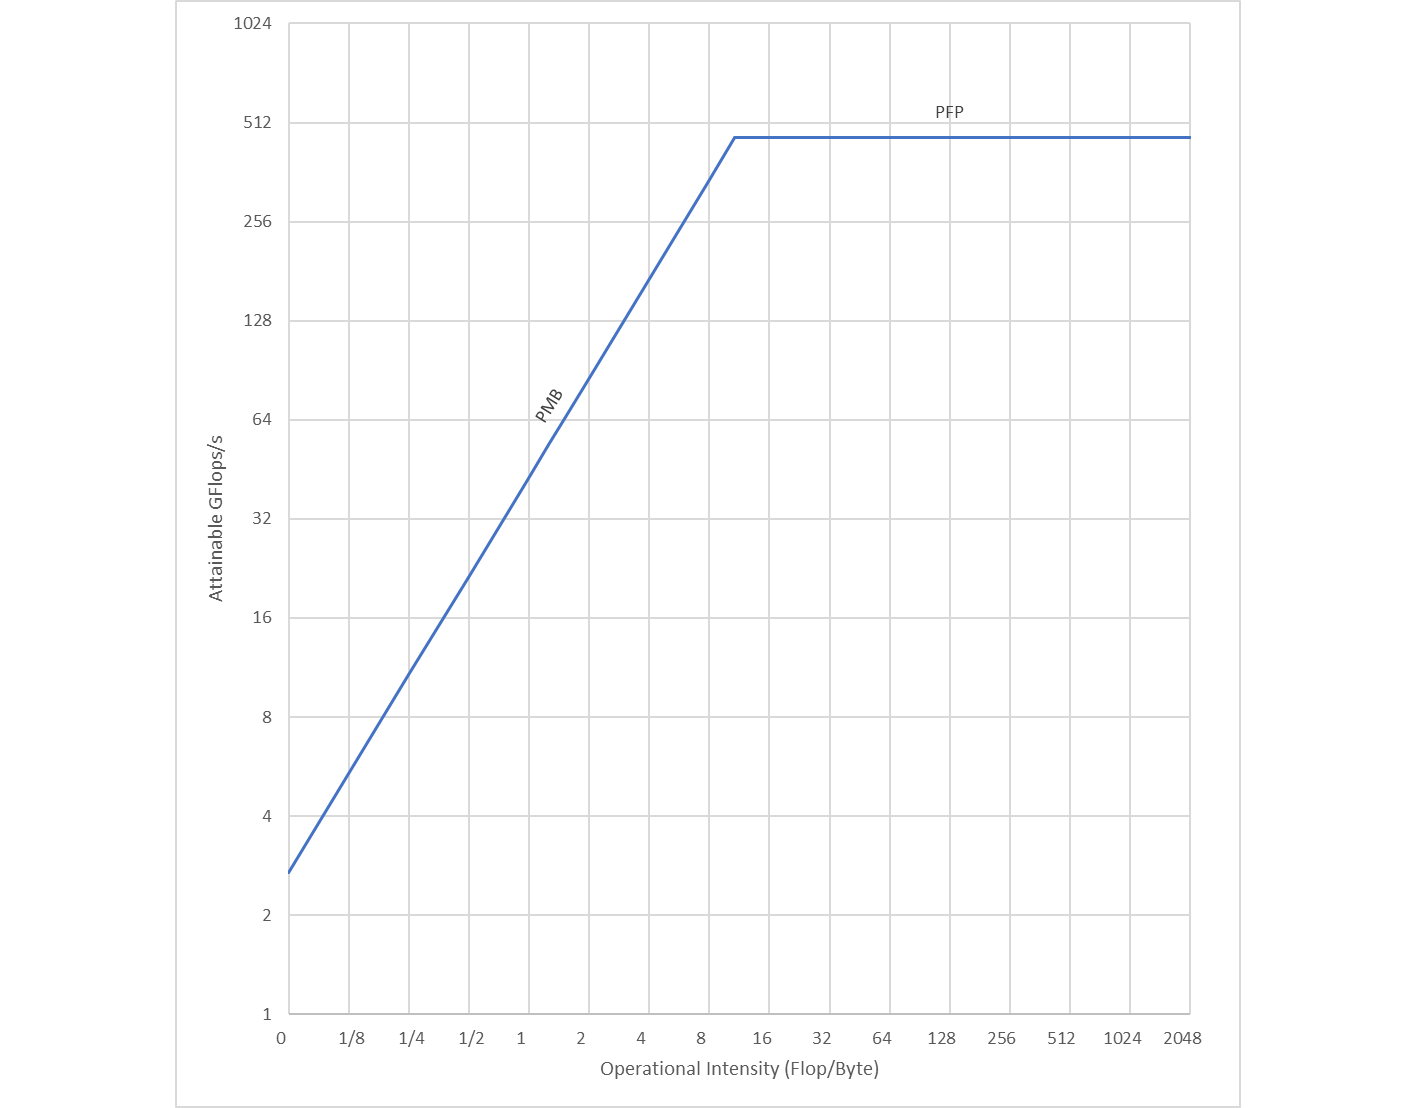
\includegraphics[width=\columnwidth]{xeon_roofline.png}
    \centering
    \caption{Roofline Model for the Intel Xeon E5-2695v2 processor.}
    \label{fig:xeonroofline}
\end{figure}

\subsection{Comparison}

As we can conclude the metrics regarding the performance analysis of the hardware are related to the resources it can provide. Table \ref{tab:comparison} in appendix \ref{ap:comparison} shows the main differences between the two architectures analysed above, concerning their specifications.

Also, plotting both Roofline Models next to each other in figure \ref{fig:comparison} helps to understand that the cluster node has almost 3 times more computation power than our laptop, for CPU bounded applications.

\begin{figure}[H]
    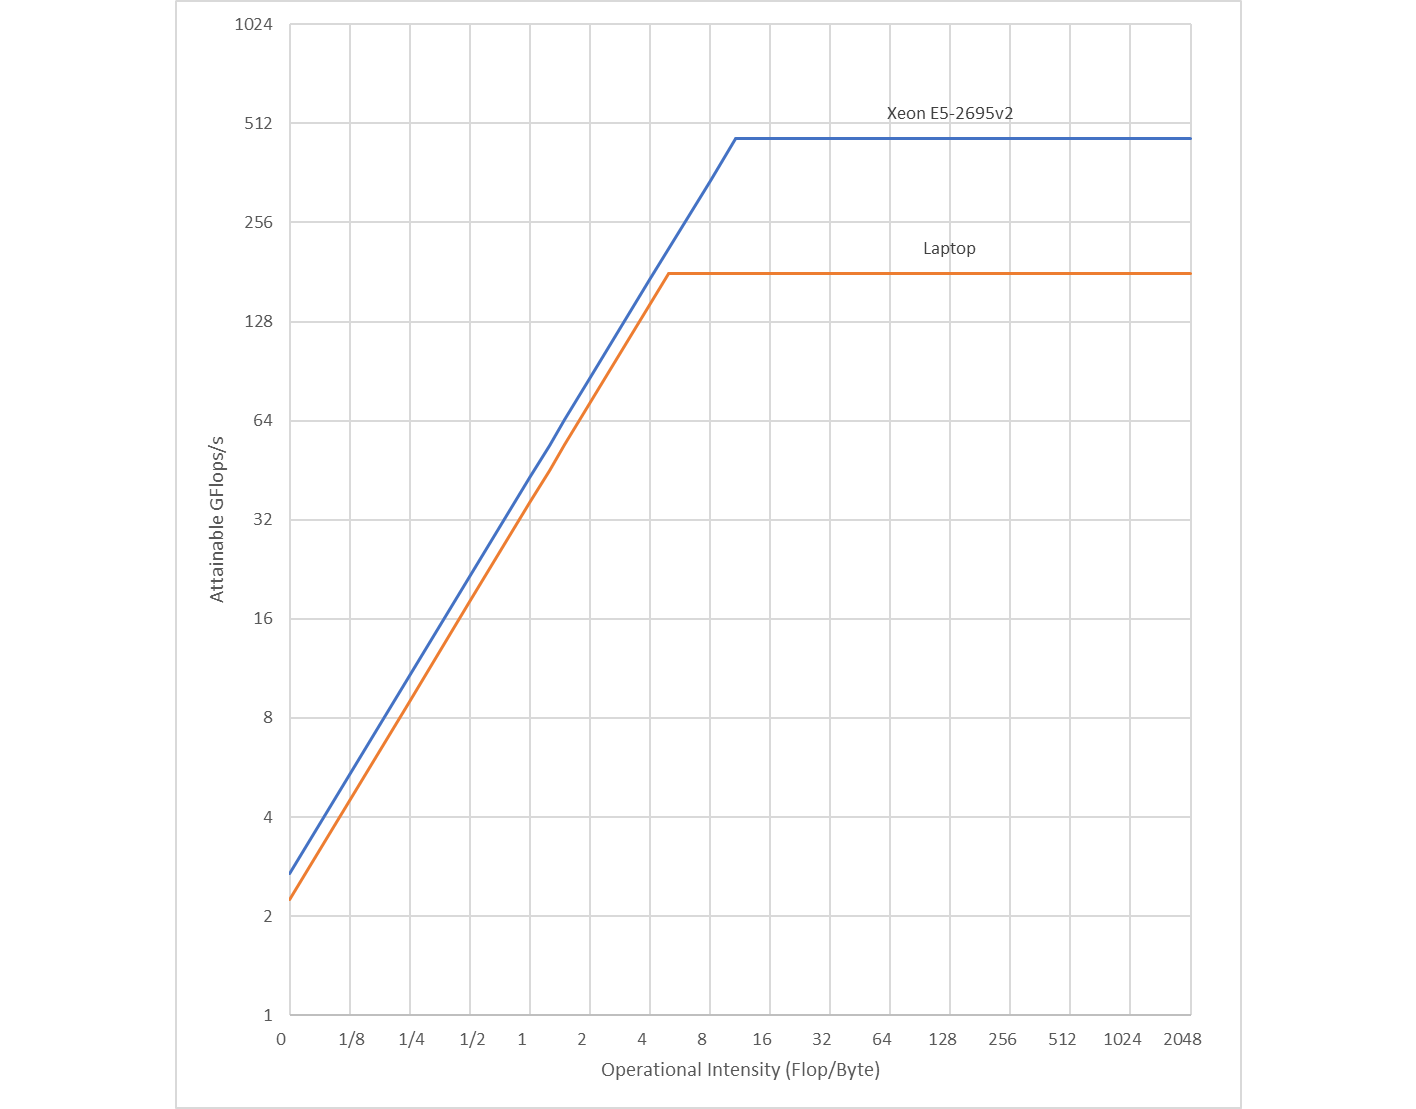
\includegraphics[width=\columnwidth]{roofline_comparison.png}
    \centering
    \caption{Intel Core i7-7700HQ vs Intel Xeon E5-2695v2 processor Roofline Model.}
    \label{fig:comparison}
\end{figure}

\section{PAPI Performance Counters}

The PAPI project successfully implements a cross-platform interface of performance hardware counters, that may provide information on how to reduce computational bottlenecks. However, in order to get relevant data from the API to our case study, we had to select a few of these events. So, to list all the available counters on the 662 nodes (PAPI version 5.5.0), we used \emph{papi\_avail} and chose the following:

\begin{itemize}
    \item \textbf{PAPI\_LD\_INS} Load instructions;
    \item \textbf{PAPI\_L1\_DCM} Level 1 data cache misses;
    \item \textbf{PAPI\_L3\_DCR} Level 3 data cache reads;
    \item \textbf{PAPI\_L3\_TCM} Level 3 cache misses;
    \item \textbf{PAPI\_L3\_TCA} Level 3 total cache accesses;
    \item \textbf{PAPI\_FP\_OPS} Floating point operations;
    \item \textbf{PAPI\_VEC\_SP} Single precision vector/SIMD instructions.
\end{itemize}

Counting these events allows us to induce certain values for important metrics, that affect the algorithm's performance. These are going to be discussed in later sections, but some of them include the miss rate for a certain level of cache, the number of RAM accesses per instruction, the floating point operations executed and the number of SIMD instructions, which are crucial when we are trying to achieve the maximum performance, on superscalar architectures.

\section{Matrix Dot-Product Algorithm Analysis}

Following the analysis and the characterisation of the hardware environment, the case study that we will be applying these modelling concepts consists of the dot product of two square matrices, where:

$$C = A \times B$$

Being \textbf{A} and \textbf{B} two square matrices of size $\textbf{N} \times \textbf{N}$ and \textbf{C} the result of the dot product between them.

\subsection{First Implementations}

The first implementations of the algorithm followed the standard three nested loop for the indexes \emph{i}, \emph{j} and \emph{k}, where \emph{i} represents the rows and \emph{j} represent the columns of the matrices.

The main changes occur when the order of the indexes is changed, producing different access patterns to the elements of the matrices.

However, when the accesses are by column, there will be a negative impact on the performance, because the matrices are stored row-wisely in memory.

This applies to the \textbf{IJK} version since the result stored in the \textbf{C} matrix is computed with a line of the matrix \textbf{A} and a column of the matrix \textbf{B}.  To address this issue, we transposed the matrix \textbf{B} to correct the access, now being row-wise.

This also occurs for the \textbf{JKI} version of the computation, since the result is iterated column-wise. So, as seen above, we changed the solution to perform the transposition of the matrices \textbf{A} and \textbf{B}, before the multiplication part of it, and \textbf{C} in the end.

\subsection{Input Data Structure}

In order to analyse the code execution on a single core of the multicore \emph{662} node, four different data set sizes were defined, based on equation \ref{eq:input}, to fit on each cache level. It was also taken into consideration choosing powers of two, from the range of values obtained by that equation. The results can be found in table \ref{tab:datasetsizes}.

\begin{equation} \label{eq:input}
    Cache Size \geqslant size^{2} \times sizeof(float) \times 3
\end{equation}

\begin{table}[ht]
\begin{tabular}{|l|l|}
\hline
Fitting Level of The Hierarchy & Size                            \\ \hline
L1 Cache                       & 32 x 32     \\ \hline
L2 Cache                       & 128 x 128   \\ \hline
L3 Cache                       & 1024 x 1024 \\ \hline
External RAM                   & 2048 x 2048 \\ \hline
\end{tabular}
\caption{Data set sizes.}
\label{tab:datasetsizes}
\end{table}

\subsection{Execution Time Measurements}

Having implemented all the of the solutions discussed above and selected the sizes for the input data sets, we measured the execution time, for each of the algorithms.

For each execution a validation test was performed to ensure that the implementation was correct. This was accomplished by verifying if all resulting columns of the product $\textbf{A} \times \textbf{B}$ had the same values. However, when measuring the execution time, this step wasn't taken into count.

To have results more reproducible, we applied a k-best scheme with $K = 3$ and a 5\% tolerance, every 8 executions. The results obtained for each of the dot product implementations and its respective input size can be seen in table \ref{tab:firsttimeresults}.

\begin{table}[h]
\centering
\resizebox{\columnwidth}{!}{
\begin{tabular}{|l|l|l|l|l|} 
\hline
                                 & \textbf{32 x 32} & \textbf{128 x 128} & \textbf{1024 x 1024} & \textbf{2048 x 2048}  \\ 
\hline
\textbf{IJK~ ~ ~ ~ ~}            & 0.037            & 2.820~ ~ ~ ~ ~     & 2972.836~ ~ ~ ~ ~    & 23635.89~ ~ ~ ~ ~     \\ 
\hline
\textbf{IJK Transposed}          & 0.037~ ~ ~ ~ ~   & 2.30~ ~ ~ ~ ~      & 1139.97~ ~ ~ ~ ~     & 9067.64~ ~ ~ ~ ~      \\ 
\hline
\textbf{IKJ~ ~ ~ ~ ~}            & 0.033~ ~ ~ ~ ~   & 1.91~ ~ ~ ~ ~      & 970.51~ ~ ~ ~ ~      & 7732.51~ ~ ~ ~ ~      \\ 
\hline
\textbf{JKI~ ~ ~ ~ ~}            & 0.046~ ~ ~ ~ ~   & 7.096~ ~ ~ ~ ~     & 17431.63~ ~ ~ ~ ~    & 80917.90~ ~ ~ ~ ~     \\ 
\hline
\textbf{JKI Transposed~ ~ }~ ~ ~ & 0.036~ ~ ~ ~ ~   & 1.980~ ~ ~ ~ ~     & 993.18~ ~ ~ ~ ~      & 7851.90~ ~ ~ ~ ~      \\
\hline
\end{tabular}
}
\caption{First implementations execution time.}
\label{tab:firsttimeresults}
\end{table}

Looking at the results, we perceived that the \textbf{JKI} implementation performed the worst for all sizes of the matrices, justifying the previous statements about the inefficiency of the column-wise memory accesses. Although the differences are more perceptible for larger sizes of the matrices, even for the \textbf{32x32} it got the worst results, like we predicted. Also, we can recognise that the \textbf{IKJ} implementation performed the best for all of the sizes, although the differences are more perceptible for larger input matrices.

Regarding the \textbf{32x32} matrix size, there is not much of a difference between all of the execution times, even so, we verify what was stated above. This is due to the fact that the \textbf{32x32} matrices fit in the first level of cache, there so the data is not replaced/invalidated.

Moving to the \textbf{128x128} matrices, only the \textbf{JKI} implementation stands out for being so much higher than the others. Because this still is a smaller size, the differences between the remaining, aren't as noticeable as well.

Now for a larger size of \textbf{1024x1024}, the contrast between the solutions that used column-wise access from the ones that implemented it row-wise is more perceptible. Verifying that the \textbf{IJK} and \textbf{JKI} benefited from transposing the matrices.

Finally, for the bigger dimension of \textbf{2048x2048}, the conclusions stated above are even more evident.

\section{Analysis of the Behaviour of the Algorithms}

After measuring the execution times, we analysed the performance of the main memory accesses, the number of floating point operations and the cache behaviour, for each of the dot product implementations. These are going to be discussed in the next subsections.

\subsection{RAM Behaviour}

Considering that the 662 nodes have a 64 byte bus width, we conclude that every access to the RAM retrieves 16 floats to the cache.

Since the algorithm is implemented with three nested loops, each iterating N times and every iteration reaches an element of A, B and C, when the access pattern is row-wise, we estimate one RAM access per 16 iterations, per matrix. That is considering that a line of cache holds 16 floats.

However, this does not apply to the access pattern being column-wise so, for the purpose of estimating, we assumed that for every load of a value from a column, we access the RAM.

Taking these into consideration, we developed the following formulas to estimate the number of RAM accesses of a matrix, for each pattern:

$$\textbf{transposing a matrix} = 2N^{2}$$
$$\textbf{row-wise} = \frac{N^{2}}{L}$$
$$\textbf{column-wise} = N^{2}$$

Where $N \times N$ is the size of the matrix and $L$ is the number of floats that fit in a line of cache. Finally, to obtain the values for each implementation we designed the formulas in appendix \ref{ap:lformulas}.

Having estimated these values, these were then obtained using the PAPI counters \textbf{PAPI\_L3\_TCM} and \textbf{PAPI\_TOT\_INS}, giving us the following results:

\begin{table}[ht]
\resizebox{\columnwidth}{!}{%
\begin{tabular}{|l|l|l|l|l|}
\hline
                        & \textbf{32 x 32} & \textbf{128 x 128} & \textbf{1024 x 1024} & \textbf{2048 x 2048} \\ \hline
\textbf{IJK}            & 0,001803311      & 0,0001098          & 3,8972E-05           & 1,98544E-05          \\ \hline
\textbf{IJK Transposed} & 0,001573423      & 0,000141863        & 4,18087E-05          & 1,87154E-05          \\ \hline
\textbf{IKJ}            & 0,001353602      & 0,000132935        & 1,71935E-05          & 8,84091E-06          \\ \hline
\textbf{JKI}            & 0,002153034      & 7,40155E-05        & 8,05869E-06          & 0,0005191            \\ \hline
\textbf{JKI Transposed} & 0,002160826      & 0,000164294        & 6,38714E-05          & 5,21549E-05          \\ \hline
\end{tabular}%
}
\caption{RAM accesses per instruction.}
\label{tab:ramresults}
\end{table}

Finally, in order to measure the number of bytes transferred to and from the main memory we multiplied the each of the results obtained above by 64 since it is the number of bytes transferred on every RAM access. Doing this, we obtained the next results:

\begin{table}
\centering
\resizebox{\columnwidth}{!}{
\begin{tabular}{|l|l|l|l|l|}
\hline
                        & \textbf{32 x 32} & \textbf{128 x 128} & \textbf{1024 x 1024} & \textbf{2048 x 2048} \\ \hline
\textbf{IJK}            & 7648             & 33856              & 12598528             & 50425248             \\ \hline
\textbf{IJK Transposed} & 6720             & 38240              & 5756736              & 20594112             \\ \hline
\textbf{IKJ}            & 5696             & 35744              & 2372224              & 9749216              \\ \hline
\textbf{JKI}            & 9376             & 41472              & 12598080             & 4109140608           \\ \hline
\textbf{JKI Transposed} & 9120             & 44160              & 8804032              & 57449952             \\ \hline
\end{tabular}%
}
\caption{Data transferred to/from the RAM.}
\label{tab:ramtrafficresults}
\end{table}

\subsection{Floating Point Operations Analysis}

Next, in the behaviour analysis of the implementations, we tried to estimate the number of floating point operations executed during each dot product implementation.

Since every algorithm does two operations every iteration and the hardware has no FMA support, we predict that all implementations are going to execute $2 \times N^{3}$ operations. To verify our estimates, we tested this for the various sizes of input and implementations, giving the following results:

\begin{table}[h]
\resizebox{\columnwidth}{!}{%
\begin{tabular}{|l|l|l|l|l|}
\hline
                        & \multicolumn{1}{c|}{\textbf{32 x 32}} & \multicolumn{1}{c|}{\textbf{128 x 128}} & \multicolumn{1}{c|}{\textbf{1024 x 1024}} & \multicolumn{1}{c|}{\textbf{2048 x 2048}} \\ \hline
\textbf{IJK}            & 66267                                 & 4817848                                 & 5051118689                                & 39683603954                               \\ \hline
\textbf{IJK Transposed} & 66733,5                               & 4211814                                 & 2151443339                                & 17193516166                               \\ \hline
\textbf{IKJ}            & 65750,5                               & 4201306,5                               & 2155812135                                & 17230299574                               \\ \hline
\textbf{JKI}            & 68043,5                               & 8754926,5                               & 24426419447                               & 1,23686E+11                               \\ \hline
\textbf{JKI Transposed} & 65947                                 & 4199800                                 & 2153748279                                & 17211330368                               \\ \hline
\end{tabular}%
}
\caption{Number of floating point operations executed.}
\label{tab:fpresults}
\end{table}

With the number of single precision floating point operations and the number of bytes to transferred to/from the main memory, we are able to obtain a value for the operational intensity. Also, having the time measurements for each size and implementation, we can plot the attainable floating point performance (see appendix \ref{ap:formulas}). With this in mind, we plotted the obtained values in the Roofline Model in figure \ref{fig:plotroofline}.

\begin{figure}[H]
    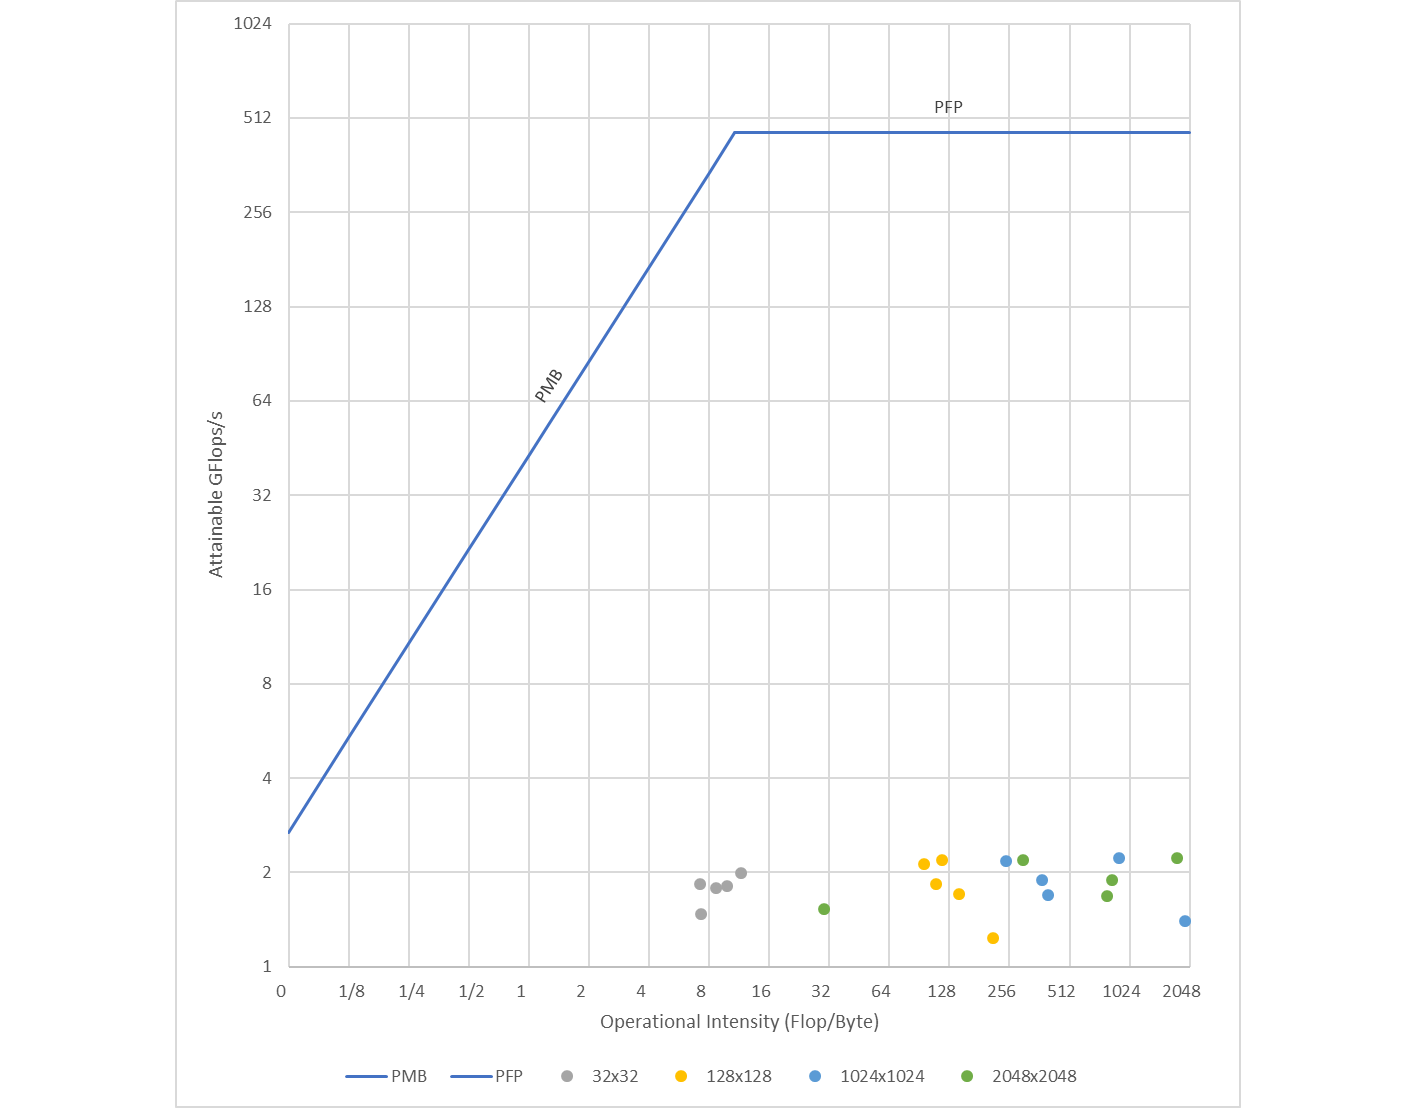
\includegraphics[width=\columnwidth]{plot_roofline.png}
    \centering
    \caption{Plotting of the obtained values.}
    \label{fig:plotroofline}
\end{figure}

As we expected, because the values for the performance obtained for the data sets (except for the smallest) are bellow the flat part of the roof, the kernel performance is compute bound.

Looking at the single core peak floating point performance, all these values are limited by the lack of vectorization. This being the next optimisation to be performed, in order to surpass that ceiling.

\subsection{Cache Behaviour}

At last, in order to have some insights into the improvements of transposing a matrix on the cache behaviour, we determined the miss rate for each cache level on implementations with and without transposing the matrices. We used the following PAPI counters and formulas for each level:

\begin{table}[ht]
\centering
\resizebox{\columnwidth}{!}{%
\begin{tabular}{|l|l|r|r|r|r|}
\hline
                            & \textbf{} & \multicolumn{1}{l|}{\textbf{32 x 32}} & \multicolumn{1}{l|}{\textbf{128 x 128}} & \multicolumn{1}{l|}{\textbf{1024 x 1024}} & \multicolumn{1}{l|}{\textbf{2048 x 2048}} \\ \hline
\multirow{3}{*}{Normal}     & L1 MR(\%) & 0,32                                  & 50,84                                   & 50,05                                     & 50,06                                     \\ \cline{2-6} 
                            & L2 MR(\%) & 47,28                                 & 0,21                                    & 99,97                                     & 99,65                                     \\ \cline{2-6} 
                            & L3 MR(\%) & 94,86                                 & 10,83                                   & 0,02                                      & 0,01                                      \\ \hline
\multirow{3}{*}{Transposed} & L1 MR(\%) & 0,31                                  & 3,25                                    & 3,18                                      & 3,15                                      \\ \cline{2-6} 
                            & L2 MR(\%) & 41,95                                 & 0,62                                    & 3,15                                      & 2,80                                      \\ \cline{2-6} 
                            & L3 MR(\%) & 93,48                                 & 71,46                                   & 4,13                                      & 1,94                                      \\ \cline{2-6} 
\end{tabular}%
}
\caption{Miss rates of the \textbf{IJK} implementation.}
\label{tab:missrates}
\end{table}

Like we foresaw, transposing the matrices improves the re-usage of the values loaded from the main memory. Although in the smaller data sets the miss rates are still high, because of the cost of transposing the matrices, the execution times are lower compared with the version that accesses the values column-wise. Proving that the algorithm benefited from this change.

\section{Optimisations}

After analysing the previous algorithms, it is time to optimise the performance of them by taking full advantage of the resources available.

We were able to see that interchanging the loops made the code access the data in the order in which they are stored. This way we improved the cache performance without affecting the number of instructions executed.

Finally, there are other optimisations we can make to enhance the execution of the algorithm, that are going to be discussed in the next sections.

\subsection{Blocking}

In order to maximise the accesses to the data loaded into the cache, before it is replaced, we applied a technique known as blocking. This optimisation consists of, instead of operating on entire rows or columns of the matrices, dividing them into squared submatrices and operating over them. This will allow us to reuse more elements, before the need to access the main memory, thus improving temporal locality.

With better use of the cache, we expect the execution time to decrease for the data sets that were requiring more accesses to the RAM.

Applying this technique to the single threaded code, that also benefited from transposing the matrices, and for the bigger size of input, we got the results in table \ref{tab:blocking}.

\begin{table}[h]
\centering
\begin{tabular}{|l|r|}
\hline
                        & \multicolumn{1}{c|}{\textbf{2048 x 2048}} \\ \hline
\textbf{IJK Transposed} & 9173                                      \\ \hline
\textbf{IKJ}            & 9175                                      \\ \hline
\textbf{JKI Transposed} & 9182                                      \\ \hline
\end{tabular}%
\caption{Execution times (in ms) of the implementations optimized with blocking and transposition.}
\label{tab:blocking}
\end{table}

\subsection{Vectorization}

Since the machine we used (\textit{662 SeARCH}) featured AVX instruction set, another optimisation that would improve the single core performance of the algorithms is vectorization through SIMD. With that in mind the team decided to switch to the Intel C++ Compiler (\textbf{ICPC}) in order to better analyse the vecotrization reports and instruct the compiler to vectorize in case it is needed.

Following that we measured the execution times for the two smaller data sets, getting the subsequent results in table \ref{tab:vec}.

\begin{table}[ht]
\centering
\begin{tabular}{|l|r|r|}
\hline
                        & \multicolumn{1}{c|}{\textbf{32x32}} & \multicolumn{1}{c|}{\textbf{128x128}} \\ \hline
\textbf{IJK Transposed} & 0,009                               & 0,59                                  \\ \hline
\textbf{IKJ}            & 0,009                               & 0,56                                  \\ \hline
\textbf{JKI Transposed} & 0,01                                & 0,609                                 \\ \hline
\end{tabular}%
\caption{Execution times (in ms) of the vectorized algorithms.}
\label{tab:vec}
\end{table}

\subsection{Multi-Core}

After analysing and optimizing the performance of the single-threaded code, it was time to take full advantage of the resources provided by the multicore devices of the 662 nodes. 

With that in mind, we adapted the vectorized code of the dot product to run efficiently on the 24 cores presented by the hardware, using \textbf{OpenMP} without Hyper Threading.

Next, we measured the execution time of the implementations, applying the same scheme as before, for the larger data set only, giving the following results in table \ref{tab:omp}.

\begin{table}[h]
\centering
\begin{tabular}{|l|r|}
\hline
                        & \multicolumn{1}{c|}{\textbf{2048x2048}} \\ \hline
\textbf{IJK Transposed} & 298,885                                 \\ \hline
\textbf{IKJ}            & 223,53                                  \\ \hline
\textbf{JKI Transposed} & 325,403                                 \\ \hline
\end{tabular}
\caption{Execution time (in ms) of the vectorized algorithms adapted to run in all cores of the multi-core devices.}
\label{tab:omp}
\end{table}

\section{Intel Knight's Landing}

In order to complement the results collected before, we also adapted the code developed for the multicore 662 nodes, to run in the Intel Knights Landing many-core server. Meaning that we selected the best performer implementation (index order i-k-j) and increased the number of threads to run in the all of the 64 cores provided by the machine, although we also tested the same implementation only with 2 threads per core of the \textbf{KNL}.

The results regarding the execution time were taken and put in table \ref{tab:final}, where we can compare with other hardware platforms.

\section{GPU Kepler}

At last, we modified the same function seen above to run in all SMX of a GPU Kepler (installed on a 662 node), rewriting the code with the CUDA paradigm in mind. This time, each thread computes one element of the result matrix,

After compiling and measuring the execution times, the results obtained can be seen in table \ref{tab:final}.

\begin{table}[h]
\resizebox{\columnwidth}{!}{%
\begin{tabular}{l|c|c|c|c|c|c|}
\cline{2-7}
                                   & \textbf{Xeon E5-2695v2}     & \multicolumn{2}{c|}{\textbf{Knight's  Landing}}           & \multicolumn{3}{c|}{\textbf{GPU  Kepler}}                                                \\ \cline{2-7} 
\textbf{}                          & \textbf{24 Threads}         & \textbf{64 Threads}         & \textbf{128 Threads}        & \textbf{Transfer to Device} & \textbf{Computation}         & \textbf{Transfer to Host}   \\ \hline
\multicolumn{1}{|l|}{\textbf{IKJ}} & \multicolumn{1}{r|}{223,53} & \multicolumn{1}{r|}{290,43} & \multicolumn{1}{r|}{164,38} & \multicolumn{1}{r|}{14,26}  & \multicolumn{1}{r|}{140,35} & \multicolumn{1}{r|}{9,9223} \\ \hline
\end{tabular}%
}
\caption{Execution times (in ms) of the same implementation in multiple platforms.}
\label{tab:final}
\end{table}

\section{Conclusions}

Switching to a multicore architecture of computing systems, the programmers confront a more diverse range of hardware capabilities. So, it is important to fully understand and analyse each resource that can be provided, in order to squeeze the maximum performance of a kernel.

In this paper, we showed how important it is to fully characterise the hardware platform environment, developing the Roofline Model, in order to get insights into the performance of a given kernel. 

This allied with the PAPI profiling API, allowed us to develop strategies to overcome the bottlenecks and optimise the performance of the matrix multiplication kernel.

These approaches include correcting the use of cache, taking advantage of SIMD instruction sets and adapting the code to run efficiently on all cores.

%----------------------------------------------------------------------------------------
%	REFERENCE LIST
%----------------------------------------------------------------------------------------

\printbibliography

%----------------------------------------------------------------------------------------
%	Appendices
%----------------------------------------------------------------------------------------

\newpage
\onecolumn
\begin{appendices}
\section{Appendix}

\subsection{}
\label{ap:comparison}

\begin{table}[ht]
\resizebox{\columnwidth}{!}{%
\begin{tabular}{|l|r|l|r|}
\hline
\multicolumn{2}{|c|}{\textbf{Intel® Core™ i7-7700HQ Processor}}                          & \multicolumn{2}{c|}{\textbf{Intel Xeon Processor E5-2695 v2}}                             \\ \hline
Code Name                           & Kaby Lake                                          & Code Name                           & Ivy Bridge EP                                       \\ \hline
\multicolumn{2}{|c|}{\textbf{Essentials}}                                                & \multicolumn{2}{c|}{\textbf{Essentials}}                                                  \\ \hline
Vertical Segment                    & Mobile                                             & Vertical Segment                    & Server                                              \\ \hline
Processor Number                    & i7-7700HQ                                          & Processor Number                    & E5-2695V2                                           \\ \hline
\multicolumn{2}{|c|}{\textbf{Performance}}                                               & \multicolumn{1}{c|}{Performance}    &                                                     \\ \hline
\# of Cores                         & 4                                                  & \# of Cores                         & 12                                                  \\ \hline
\# of Threads                       & 8                                                  & \# of Threads                       & 24                                                  \\ \hline
Processor Base Frequency            & 2.80 GHz                                           & Processor Base Frequency            & 2.40 GHz                                            \\ \hline
Max Turbo Frequency                 & 3.80 GHz                                           & Max Turbo Frequency                 & 3.20 GHz                                            \\ \hline
Bus Speed                           & 8 GT/s DMI                                         & Bus Speed                           & 8 GT/s QPI                                          \\ \hline
\multicolumn{2}{|c|}{\textbf{Memory Specifications}}                                     & \multicolumn{2}{c|}{\textbf{Memory Specifications}}                                       \\ \hline
\multirow{2}{*}{Level 1 cache size} & 4 x 32 KB 8-way set associative instruction caches & \multirow{2}{*}{Level 1 cache size} & 12 x 32 KB 8-way set associative instruction caches \\ \cline{2-2} \cline{4-4} 
                                    & 4 x 32 KB 8-way set associative data caches        &                                     & 12 x 32 KB 8-way set associative data caches        \\ \hline
Level 2 cache size                  & 4 x 256 KB 4-way set associative caches            & Level 2 cache size                  & 12 x 256 KB 8-way set associative caches            \\ \hline
Level 3 cache size                  & 6 MB 12-way set associative shared cache           & Level 3 cache size                  & 30 MB 20-way set associative shared cache           \\ \hline
Memory Types                        & DDR4-2400, LPDDR3-2133, DDR3L-1600                 & Memory Types                        & DDR3 800/1066/1333/1600/1866                        \\ \hline
Max \# of Memory Channels           & 2                                                  & Max \# of Memory Channels           & 4                                                   \\ \hline
Max Memory Bandwidth                & 37.5 GB/s                                          & Max Memory Bandwidth                & 59.7 GB/s                                           \\ \hline
\multicolumn{2}{|c|}{\textbf{Advanced Technologies}}                                     & \multicolumn{2}{c|}{\textbf{Advanced Technologies}}                                       \\ \hline
Intel® 64 ‡                         & Yes                                                & Intel® 64 ‡                         & Yes                                                 \\ \hline
Instruction Set                     & 64-bit                                             & Instruction Set                     & 64-bit                                              \\ \hline
Instruction Set Extensions          & Intel® AVX                                         & Instruction Set Extensions          & Intel® AVX                                          \\ \hline
FMA Support                         & v3                                                 & FMA Support                         & n/a                                                 \\ \hline
\end{tabular}%
}
\caption{Intel core i7-7700HQ vs Intel Xeon E5-2965v2 specifications.}
\label{tab:comparison}
\end{table}

\subsection{Estimates of Load Instructions of Matrix Multiplication}
\label{ap:lformulas}

The next formulas were derived with the intent to estimate the number of accesses to the main memory in the dot product matrix multiplication.

\begin{equation} \label{eq:ijk}
\textbf{IJK} = \frac{N^{2}}{L} + N^{2} + \frac{N^{2}}{L} = N^{2} + \frac{2N^{2}}{L}
\end{equation}

\begin{equation} \label{eq:ijktr}
\textbf{IJKTr} = 2N^{2} + \frac{N^{2}}{L} + \frac{N^{2}}{L} + \frac{N^{2}}{L} = 2N^{2} + \frac{3N^{2}}{L}
\end{equation}

\begin{equation} \label{eq:ikj}
\textbf{IKJ} = \frac{N^{2}}{L} + \frac{N^{2}}{L} + \frac{N^{2}}{L} = \frac{3N^{2}}{L}
\end{equation}

\begin{equation} \label{eq:jki}
\textbf{JKI} = N^{2} + N^{2} + N^{2} = 3N^{2}
\end{equation}

\begin{equation} \label{eq:jkitr}
\textbf{JKITr} = 2N^{2} + 2N^{2} + 2N^{2} + \frac{N^{2}}{L} + \frac{N^{2}}{L} + \frac{N^{2}}{L} = 6N^{2} + \frac{3N^{2}}{L}
\end{equation}

\subsection{Matrix Multiplication Kernel PAPI Readings}
\label{ap:formulas}

With these counters, we were able to derive the subsequent formulas so to get insights on metrics relevant to the performance of the kernel.

\begin{equation} \label{eq:l1mr}
\textbf{L1 MR} = \frac{PAPI\_L1\_DCM}{PAPI\_LD\_INS} 
\end{equation}

\begin{equation} \label{eq:l2mr}
\textbf{L2 MR} = \frac{PAPI\_L2\_TCM}{PAPI\_L1\_DCM}
\end{equation}

\begin{equation} \label{eq:l3mr}
\textbf{L3 MR} = \frac{PAPI\_L3\_TCM}{PAPI\_L2\_DCM}
\end{equation}

\begin{equation} \label{eq:ramacc}
    \textbf{\#RAM Accesses} = PAPI\_L3\_TCM
\end{equation}

\begin{equation} \label{eq:rambytes}
\textbf{\#Bytes TransferredRAM} = \#RAM Accesses \times 64
\end{equation}

\begin{equation}
\textbf{\#FP Operations} = PAPI\_FP\_OPS
\end{equation}

\begin{equation}
    \textbf{OpIntensity} = \frac{\#FP Operations}{\#Bytes Transferred_{RAM}}
\end{equation}

\begin{equation}
    \textbf{Performance} = \frac{\#FP Operations}{ExecutionTime \times 10^{5}}
\end{equation}

\end{appendices}

%----------------------------------------------------------------------------------------

\end{document}
